\documentclass{article}
\usepackage[margin=1in]{geometry}
\usepackage{enumitem}
\usepackage{setspace}
\usepackage{amsmath}
\usepackage{amssymb}
\usepackage{physics}
\usepackage{graphicx}

\title{Math 132 Homework 2}
\date{10/14/2020}
\author{Jiaping Zeng}

\begin{document}
\setstretch{1.35}
\maketitle

\begin{itemize}
    \item [1.3.33] $z^4=i$\\
          \textbf{Answer: } $z^4=i\implies z^4=\cos\frac{\pi}{2}+i\sin\frac{\pi}{2}$, then we have \\$z_1=\cos\frac{\pi}{8}+i\sin\frac{\pi}{8}=\frac{\sqrt{2+\sqrt{2}}}{2}+\frac{\sqrt{2-\sqrt{2}}}{2}i$ (principal root)\\$z_2=\cos\frac{5\pi}{8}+i\sin\frac{5\pi}{8}=-\frac{\sqrt{2+\sqrt{2}}}{2}+\frac{\sqrt{2-\sqrt{2}}}{2}i$\\$z_3=\cos\frac{9\pi}{8}+i\sin\frac{9\pi}{8}=-\frac{\sqrt{2+\sqrt{2}}}{2}-\frac{\sqrt{2-\sqrt{2}}}{2}i$\\$z_4=\cos\frac{13\pi}{8}+i\sin\frac{13\pi}{8}=\frac{\sqrt{2+\sqrt{2}}}{2}-\frac{\sqrt{2-\sqrt{2}}}{2}i$
          \begin{center}
              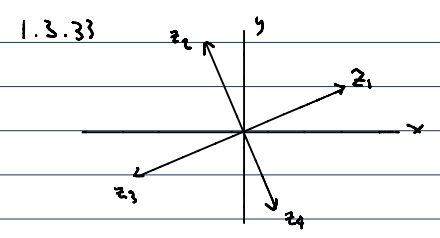
\includegraphics[width=2in]{1-3-33.png}
          \end{center}
    \item [1.4.30] Find the image of the set $S=\{z:\abs{z}\leq 1\}$ under the mapping $f(z)=z+\bar{z}$.\\
          \textbf{Answer: } Let $z=x+yi$, then $f(z)=z+\bar{z}=(x+yi)+(x-yi)=2x=2\Re z$. Therefore $f[S]$ "squishes" the disk with radius 1 $S$ to a segment from $-2$ to $2$ on the real axis.
          \begin{center}
              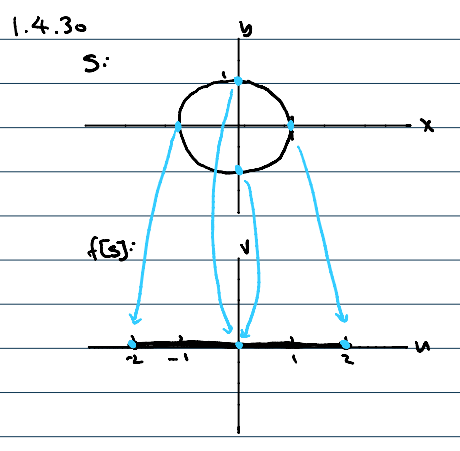
\includegraphics[width=2in]{1-4-30.png}
          \end{center}
    \item [1.4.32] $S=\{z:\abs{z}\geq 1\}$\\
          \textbf{Answer: } Let $z=r(\cos\theta+i\sin\theta)$, then $\abs{z}\geq 1\implies r\geq 1\implies\frac{1}{r}\leq 1$. Therefore $f[S]=\{z:\abs{z}\leq 1\}$.
          \begin{center}
              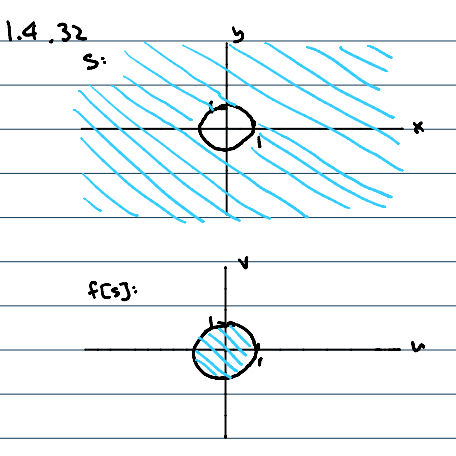
\includegraphics[width=2in]{1-4-32.png}
          \end{center}
    \item [1.6.29] $\sin(z_1+z_2)=\sin z_1\cos z_2+\cos z_1\sin z_2$\\
          \textbf{Answer: } We can expand the right hand side by definition of complex sine and cosine functions as follows:\\$\sin z_1\cos z_2+\cos z_1\sin z_2$\\$=\frac{e^{iz_1}-e^{-iz_1}}{2i}\cdot\frac{e^{iz_2}+e^{-iz_2}}{2}+\frac{e^{iz_1}+e^{-iz_1}}{2}\cdot\frac{e^{iz_2}-e^{-iz_2}}{2i}$\\$=\frac{(e^{iz_1}-e^{-iz_1})(e^{iz_2}+e^{-iz_2})}{4i}+\frac{(e^{iz_1}+e^{-iz_1})(e^{iz_2}-e^{-iz_2})}{4i}$\\$=\frac{e^{iz_1}\cdot e^{iz_2}+e^{iz_1}\cdot e^{-iz_2}-e^{-iz_1}\cdot e^{iz_2}-e^{-iz_1}\cdot e^{-iz_2}}{4i}+\frac{e^{iz_1}\cdot e^{iz_2}-e^{iz_1}\cdot e^{-iz_2}+e^{-iz_1}\cdot e^{iz_2}-e^{-iz_1}\cdot e^{-iz_2}}{4i}$\\$=\frac{e^{i(z_1+z_2)}+e^{i(z_1-z_2)}-e^{i(-z_1+z_2)}-e^{i(-z_1-z_2)}}{4i}+\frac{e^{i(z_1+z_2)}-e^{i(z_1-z_2)}+e^{i(-z_1+z_2)}-e^{i(-z_1-z_2)}}{4i}$\\$=\frac{2e^{i(z_1+z_2)}-2e^{i(-z_1-z_2)}}{4i}$\\$=\frac{e^{i(z_1+z_2)}-e^{i(-z_1-z_2)}}{2i}$\\$=\sin(z_1+z_2)$
    \item [1.7.2] $z=-3-3i$\\
          \textbf{Answer: } $\log z=\ln\abs{z}+i\arg z=\ln\sqrt{18}+i(\frac{5\pi}{4}+2k\pi), k\in\mathbb{Z}$
    \item [1.7.3] $z=5e^{i\frac{\pi}{7}}$\\
          \textbf{Answer: } $\log z=\ln\abs{z}+i\arg z=\ln 5+i(\frac{\pi}{7}+2k\pi), k\in\mathbb{Z}$
    \item [1.7.19]
          \begin{itemize}
              \item [(a)] Compute $\text{Log}(e^{i\pi})$, $\text{Log}(e^{3i\pi})$, and $\text{Log}(e^{5i\pi})$.\\
                    \textbf{Answer: }\\
                    $\text{Log}(e^{i\pi})=\ln\abs{z}+i\text{Arg }z=\ln 1+i\pi$\\
                    $\text{Log}(e^{3i\pi})=\text{Log}(\cos 3\pi+i\sin 3\pi)=\text{Log}(\cos\pi+i\sin\pi)=\text{Log}(e^{i\pi})=\ln 1+i\pi$\\
                    $\text{Log}(e^{5i\pi})=\text{Log}(\cos 5\pi+i\sin 5\pi)=\text{Log}(\cos\pi+i\sin\pi)=\text{Log}(e^{i\pi})=\ln 1+i\pi$
              \item [(b)] Show that $\text{Log}(e^z)=z$ if and only if $-\pi<\Im z\leq\pi$.\\
                    \textbf{Answer: } Let $z=x+iy$, then $\Im z=y$;
                    \begin{itemize}
                        \item [$\Rightarrow$:] If $\text{Log}(e^z)=z$, by definition of Log we have $\ln\abs{z}+i\text{Arg }z=z$. Since $\text{Arg }z=\text{Arg }e^{x+iy}=y=\Im z$, we must have $-\pi<\text{Arg }z<\pi\implies -\pi<\Im z<\pi$ by definition of principal value.
                        \item [$\Leftarrow$:] If $-\pi<\Im z\leq\pi$, we can evaluate $\text{Log}(e^z)$ as follows: $\text{Log}(e^z)=\text{Log}(e^x\cdot e^{iy})=\ln\abs{e^x\cdot e^{iy}}+i\text{Arg }(e^x\cdot e^{iy})=\ln\abs{e^x}+iy=x+iy=z$.
                    \end{itemize} 
          \end{itemize}
    \item [1.7.24] $(1+i)^{3+i}$\\
          \textbf{Answer: } $(1+i)^{3+i}=e^{(3+i)\text{Log}(1+i)}=e^{(3+i)\text{Log}(\sqrt{2}e^{i\frac{\pi}{4}})}=e^{(3+i)(\ln\sqrt{2}+i\frac{\pi}{4})}=e^{3\ln\sqrt{2}-\frac{\pi}{4}+i(\frac{3\pi}{4}+\ln\sqrt{2})}$
    \item [P1] Find and plot all $z\in\mathbb{C}$ such that $(z-3+i)^3=-125i$.\\
          \textbf{Answer: } Let $w=z-3+i$, then we have $w^3=-125i\implies w^3=-125(\cos\frac{\pi}{2}+i\sin\frac{\pi}{2})$. Then the roots are\\
          $w_1=-5(\cos\frac{\pi}{6}+i\sin\frac{\pi}{6})=-\frac{5\sqrt{3}}{2}-\frac{5}{2}i$\\
          $w_2=-5(\cos\frac{5\pi}{6}+i\sin\frac{5\pi}{6})=\frac{5\sqrt{3}}{2}-\frac{5}{2}i$\\
          $w_3=-5(\cos\frac{9\pi}{6}+i\sin\frac{9\pi}{6})=5i$\\
          By substitution we have\\
          $z_1=w_1+3-i=3-\frac{5\sqrt{3}}{2}-\frac{7}{2}i$\\
          $z_2=w_2+3-i=3+\frac{5\sqrt{3}}{2}-\frac{7}{2}i$\\
          $z_3=w_3+3-i=3+4i$
    \item [P2] In each part, express $f(z)$ in the form $u(x,y)+iv(x,y)$ where $u$ and $v$ are the real and imaginary parts of $f$:
          \begin{itemize}
              \item [(a)] $f(z)=z^3$\\
                    \textbf{Answer: } Let $z=x+iy$, then $f(z)=z^3=(x+iy)^3=x^3+3ix^2y-3xy^2-iy^3=(x^3-3xy^2)+i(3x^2y-y^3)$. Then $u(x,y)=x^3-3xy^2$ and $v(x,y)=3x^2y-y^3$.
              \item [(b)] $f(z)=\abs{z}^3$\\
                    \textbf{Answer: } Since $\abs{z}=\abs{x+iy}\in\mathbb{R}$, we have $u(x,y)=\abs{x+iy}^3$ and $v(x,y)=0$.
          \end{itemize}
    \item [P3] Sketch each of the following regions $D$ and its image under the exponential map $w=e^z$. Indicate the images of horizontal and vertical lines in your sketch.\begin{itemize}
              \item [(a)] The vertical strip $D=\{z\in\mathbb{C}\mid 0<\Re(z)<1\}$.\\
                    \begin{center}
                        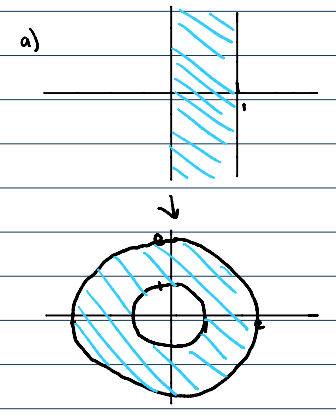
\includegraphics[width=2in]{p2a.png}
                    \end{center}
              \item [(b)] The horizontal strip $D=\{z\in\mathbb{C}\mid\frac{5\pi}{3}<\Im(z)<\frac{8\pi}{3}\}$.\\
                    \begin{center}
                        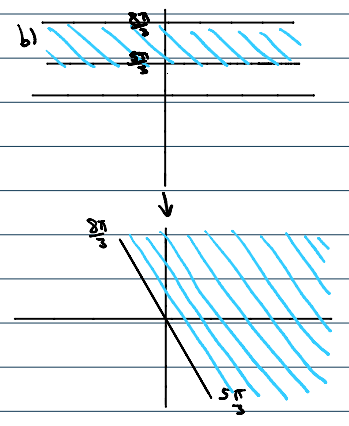
\includegraphics[width=2in]{p2b.png}
                    \end{center}
              \item [(c)] The rectangle $D=\{z\in\mathbb{C}\mid 0<\Re(z)<1,0<\Im(z)<\frac{\pi}{4}\}$.\\
                    \begin{center}
                        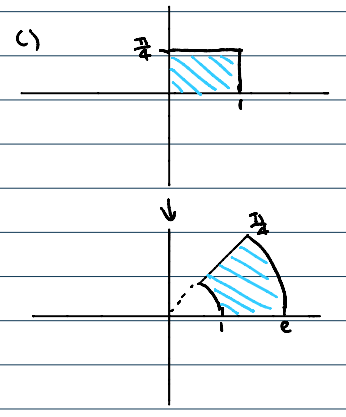
\includegraphics[width=2in]{p2c.png}
                    \end{center}
          \end{itemize}
    \item [P4] Find all values of the complex power $i^i$.\\
          \textbf{Answer: } $i^i=e^{i\log i}=e^{i\log (\ln 1+i\frac{\pi}{2})}=e^{-\frac{\pi}{2}+2k\pi}, k\in\mathbb{Z}$
\end{itemize}
\end{document}